\documentclass[tikz]{standalone}

\usetikzlibrary{calc}

\def\layersep{3cm}
\newcommand\nn[1]{
    % Input layer
    \foreach \y in {1,...,2}
        \node[neuron, fill=green!40] (i\y-#1) at (0,\y+1) {$i\y$};

    % Hidden layer
    \foreach \y in {1,...,4}
        \path node[neuron, fill=blue!40] (h\y-#1) at (\layersep,\y) {$h\y$};

    % Output node
    \node[neuron, fill=red!40] (o-#1) at (2*\layersep,2.5) {$o$};

    % Connect every node in the input layer with every node in the hidden layer.
    \foreach \source in {1,...,2}
        \foreach \dest in {1,...,4}
            \path (i\source-#1) edge (h\dest-#1);

    % Connect every node in the hidden layer with the output layer
    \foreach \source in {1,...,4}
        \path (h\source-#1) edge (o-#1);
}

\begin{document}
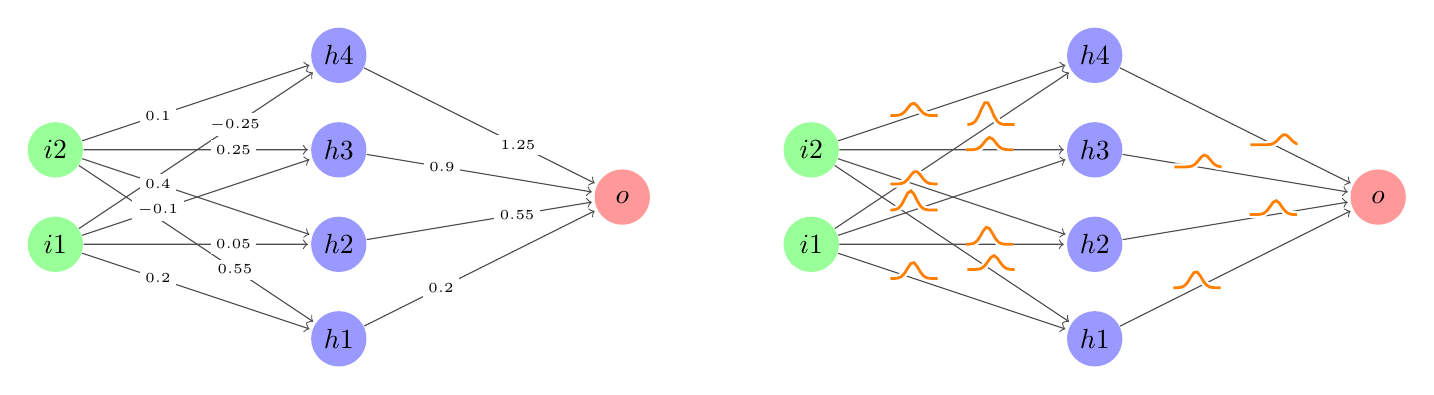
\begin{tikzpicture}[
    scale=1.2,
    shorten >=1pt,->,draw=black!70, node distance=\layersep,
    neuron/.style={circle,fill=black!25,minimum size=20,inner sep=0},
    edge/.style 2 args={pos={(mod(#1+#2,2)+1)*0.33}, font=\tiny},
    distro/.style 2 args={
        edge={#1}{#2}, node contents={}, minimum size=0.6cm, path picture={\draw[double=orange,white,thick,double distance=1pt,shorten >=0pt] plot[variable=\t,domain=-1:1,samples=51] ({\t},{0.2*exp(-100*(\t-0.05*(#1-1))^2 - 3*\t*#2))});}
      },
    weight/.style 2 args={
        edge={#1}{#2}, node contents={\pgfmathparse{0.35*#1-#2*0.15}\pgfmathprintnumber[fixed]{\pgfmathresult}}, fill=white, inner sep=2pt
      }
  ]
  \nn{regular}

  \begin{scope}[xshift=8cm]
    \nn{bayes}
  \end{scope}

  % Draw weights for all regular edges.
  \foreach \i in {1,...,2}
  \foreach \j in {1,...,4}
  \path (i\i-regular) -- (h\j-regular) node[weight={\i}{\j}];
  \foreach \i in {1,...,4}
  \path (h\i-regular) -- (o-regular) node[weight={\i}{1}];

  % Draw distros for all Bayesian edges.
  \foreach \i in {1,...,2}
  \foreach \j in {1,...,4}
  \path (i\i-bayes) -- (h\j-bayes) node[distro={\i}{\j}];
  \foreach \i in {1,...,4}
  \path (h\i-bayes) -- (o-bayes) node[distro={\i}{1}];
\end{tikzpicture}
\end{document}
